\chapter{ Computed Torque controllers}

In this chapter multiple variations of computed torque controllers will be developed and applied to the just verified model of the robot. 
In general computed torque controllers are nonlinear ones, which are linearizing the errors of the system, so that a linear controller can be applied. Therefore the previously deducted model will be used. First the error system needs to be defined: 

\begin{gather*}
\mathbf{e} = \mathbf{q}_D - \mathbf{q}\\
\dot{\mathbf{e}} = \dot{\mathbf{q}}_D - \dot{\mathbf{q}}\\
\ddot{\mathbf{e}} = \ddot{\mathbf{q}}_D - \ddot{\mathbf{q}}
%\label{eq:eq1}
\intertext{where:}
\begin{tabular}{>{$}l<{$} @{${}:{}$} l}
\mathbf{e} & error vector\\
\mathbf{q}_D & vector with reference trajectories for each joint
\end{tabular}\nonumber
\end{gather*}

Substituting the robot dynamic equation \eqref{eq:dynamic equation} into the acceleration vector $\ddot{\mathbf{q}}$, results in:
\begin{equation*}
\ddot{\mathbf{e}} = \ddot{\mathbf{q}}_D - \mathbf{M}^{-1}\left(\tau - \mathbf{v} - \mathbf{g}\right) + \mathbf{M}^{-1}\tau_D
\end{equation*}
Defining $\mathbf{u} = \ddot{\mathbf{q}}_D - \mathbf{M}^{-1}\left(\tau - \mathbf{v} - \mathbf{g}\right)$ and $\mathbf{w} = \mathbf{M}^{-1}\tau_D$ results in the following linear system
\begin{equation*}
\left(\begin{array}{c}
\dot{\mathbf{e}} \\ \ddot{\mathbf{e}}
\end{array}\right) = \left(\begin{array}{cc}
\mathbf{0} & \mathbf{I} \\
\mathbf{0} & \mathbf{0} 
\end{array}\right) \left(\begin{array}{c}
\mathbf{e} \\ \dot{\mathbf{e}}
\end{array}\right) + \left(\begin{array}{c}
\mathbf{0} \\ \mathbf{I}
\end{array}\right) \mathbf{u} + \left(\begin{array}{c}
\mathbf{0} \\ \mathbf{I}
\end{array}\right) \mathbf{w}
\end{equation*}
As the actual input of the robot arm is not the input $\mathbf{u}$, but the motor torque $\tau$, $\mathbf{u} = \ddot{\mathbf{q}}_D - \mathbf{M}^{-1}\left(\tau - \mathbf{v} - \mathbf{g}\right)$ needs to be solved for $\tau$:
\begin{equation}
\tau = \mathbf{M}(\ddot{\mathbf{q}}_D - \mathbf{u}) + \mathbf{v} + \mathbf{g}
\label{eq:ch2_ctlaw}
\end{equation}

The \eqref{eq:ch2_ctlaw} is the inner control low, which linearizes the robot to a linear double integrator. The closed loop dynamics of the robot can now be defined by choosing a proper control law for $\mathbf{u}$. In the figure \ref{fig:ct_overview} the control structure can be seen, with the outer controller and the inner one, which is linearizing.

\begin{figure}[]
	\centering
	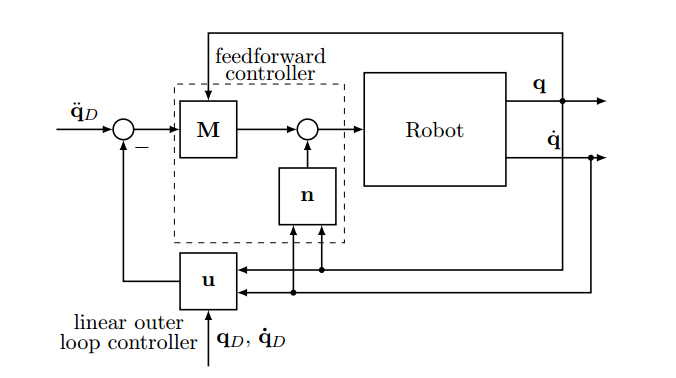
\includegraphics[width=0.85\textwidth]{pics/ct_controller.png}\\
	\caption{Schmetics of the 2DOF Robot arm}
	\label{fig:ct_overview}
\end{figure}



\section{PD-Controller}

For the PD-Controller a controller of the structure 
\begin{gather*}
\mathbf{u} = -\mathbf{K}_d \dot{\mathbf{e}} - \mathbf{K}_p \mathbf{e}
\intertext{where:}
\begin{tabular}{>{$}l<{$} @{${}:{}$} l}
\mathbf{K}_d & diagonal matrix with derivative gains \\
\mathbf{K}_p & diagonal matrix with proportional gains
\end{tabular}\nonumber
\end{gather*}
is chosen. It can be shown that the characteristic polynomial of the closed loop answer is: 

\begin{equation*}
\Delta(s) = s^2 + k_{d} s + k_{p} = 0
\end{equation*}

By comparing this polynomial to a general second order system:

\begin{equation*}
p(s) = s^2 + 2\zeta \omega_ns+{\omega_n}^2
\end{equation*}

it can be seen, that $k_{d} = 2\zeta \omega_n $ and $k_p = {\omega_n}^2$. For the frequency of the system $\omega_n$ the value 10 has been chosen. The damping factor will be changed over different simulations to show the influence of over- and under-damping.
At last another simulation will be discussed, with the initial settings for the controller but with an external distortion. In table \ref{tab:ch2_pdparams} the different settings for the four simulations can be seen.

\begin{table}[h]
	\begin{center}
		
		\label{tab:ch2_pdparams}
		\begin{tabular}{lllll}
			& & & & According \\
			& $k_{p}$ & $k_{d}$ & $\tau_D$ & Figure \\
			\midrule
			$\zeta = 1$: & 100 & 20 & $0\,\mathrm{N\,m}$ & \ref{fig:ct_pd1} \\
			$\zeta = 0.1$: & 100 & 2 & $0\,\mathrm{N\,m}$ & \ref{fig:ct_pd2} \\
			$\zeta = 10$: & 100 & 200 & $0\,\mathrm{N\,m}$ & \ref{fig:ct_pd3} \\
			$\zeta = 1$: & 100 & 20 & $1\,\mathrm{N\,m}$ & \ref{fig:ct_pd4} \\
			\bottomrule
		\end{tabular}
	\caption{Controller parameters for simulations witch PD outer loop controller}
	\end{center}
\end{table}

In figure \ref{fig:ct_pd1} the simulation results the critical damping. The error of the system for the first joint starts at zero and has a small peak around 0.01 rads; the second joint has its error peak right at the beginning with 0.1rads. The torque has rather high peaks right at the beginning but is reduced almost immediately to values around 30Nm for the first and 10Nm for the seconds joint. Wrapped up this simulation result shows that the robot arm behaves as expected. The error of the system is reduced to a minimum pretty fast, as it has been expected by a critically damped system.\\

\begin{figure}[]
	\centering
	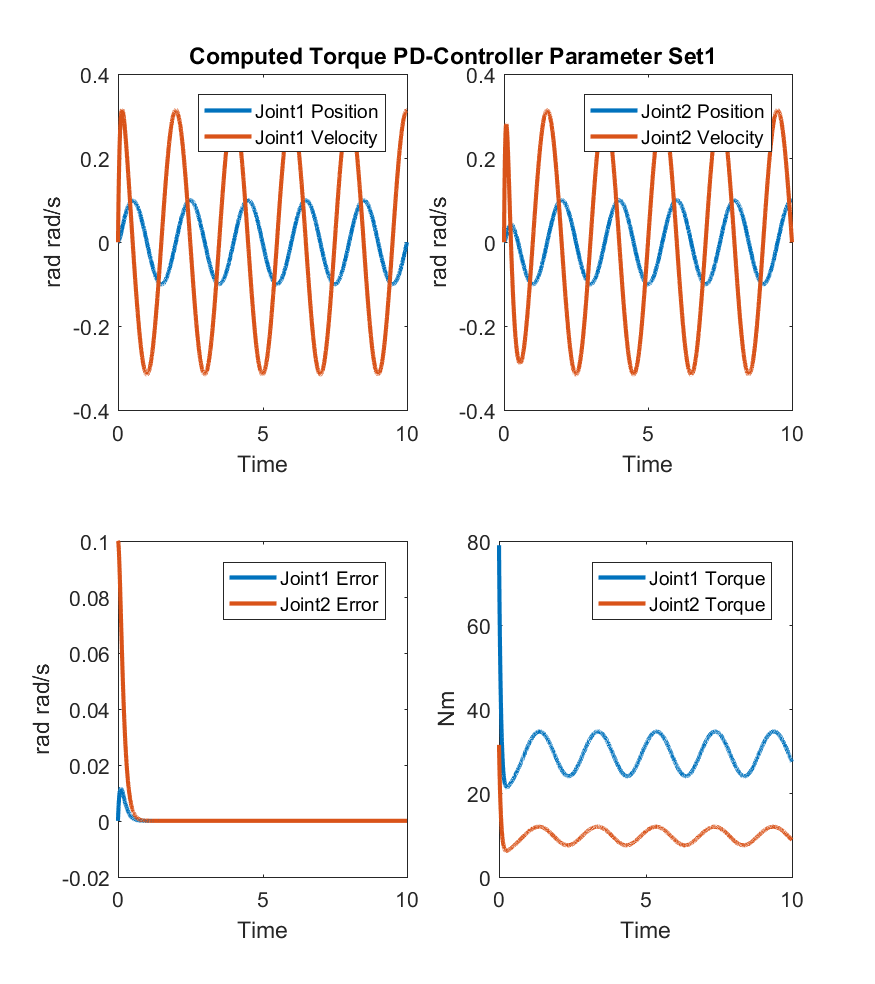
\includegraphics[width=0.85\textwidth]{pics/ComputedTorquePD-ControllerParameterSet1.png}\\
	\caption{Computed Torque PD Controller}
	\label{fig:ct_pd1}
\end{figure}

The next simulation result \ref{fig:ct_pd2} show the behavior of the system in combination with an under-damped controller. Per definition an under-damped system oscillates with a frequency, slightly different to the undamped case, until the amplitude of the oscillation gradually reaches zero. This is exactly the behavior of the robot arm. When the error is taken in observation, it can be seen that there are quite severe oscillations, in comparison the the previous simulation. The robot arm needs around 5 seconds to finally move without an position error.\\
\begin{figure}[]
	\centering
	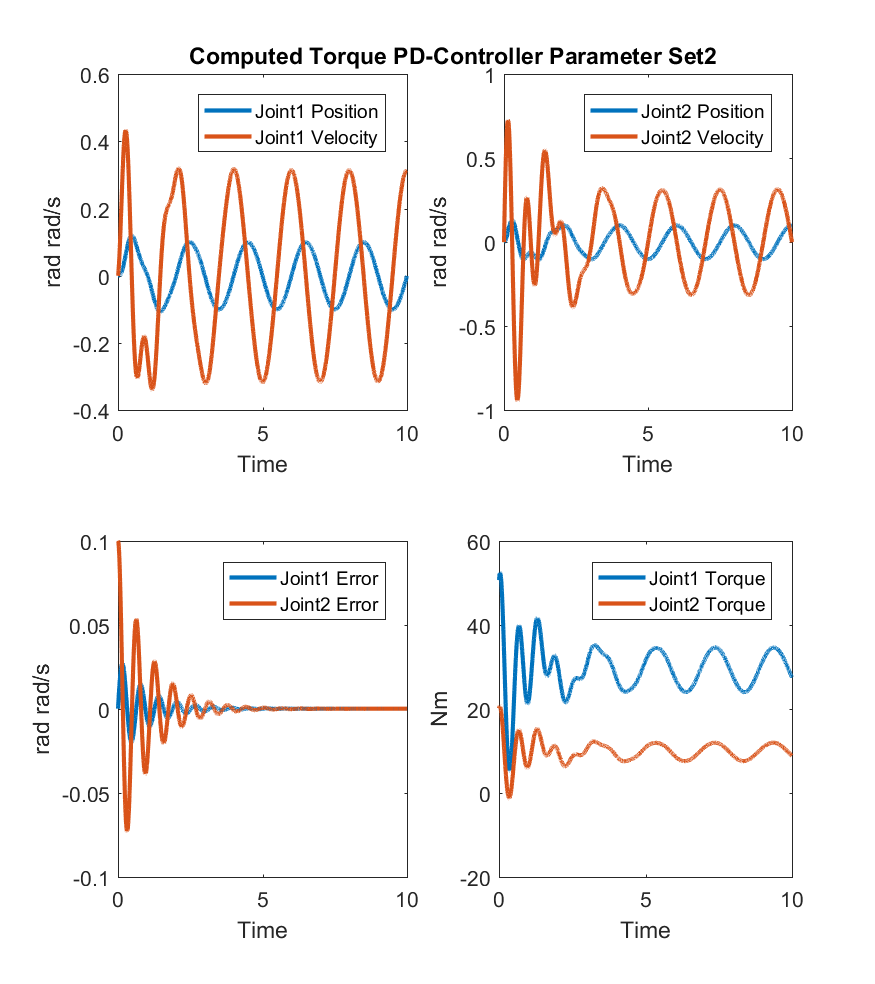
\includegraphics[width=0.85\textwidth]{pics/ComputedTorquePD-ControllerParameterSet2.png}\\
	\caption{Computed Torque PD Controller with under-damping}
	\label{fig:ct_pd2}
\end{figure}

The third simulation, which can be seen in figure \ref{fig:ct_pd3}, has a controller, which is over-damped. An over-damped controller drives the system to steady state with exponential decay without any oscillations. Exactly this behavior can be seen within the simulation results. To force the system on this trajectory, there are high torque values needed ( up to 350Nm), which makes this approach not very useful for a real world application, since there would be huge motors needed, to drive this torques.\\
\begin{figure}[]
	\centering
	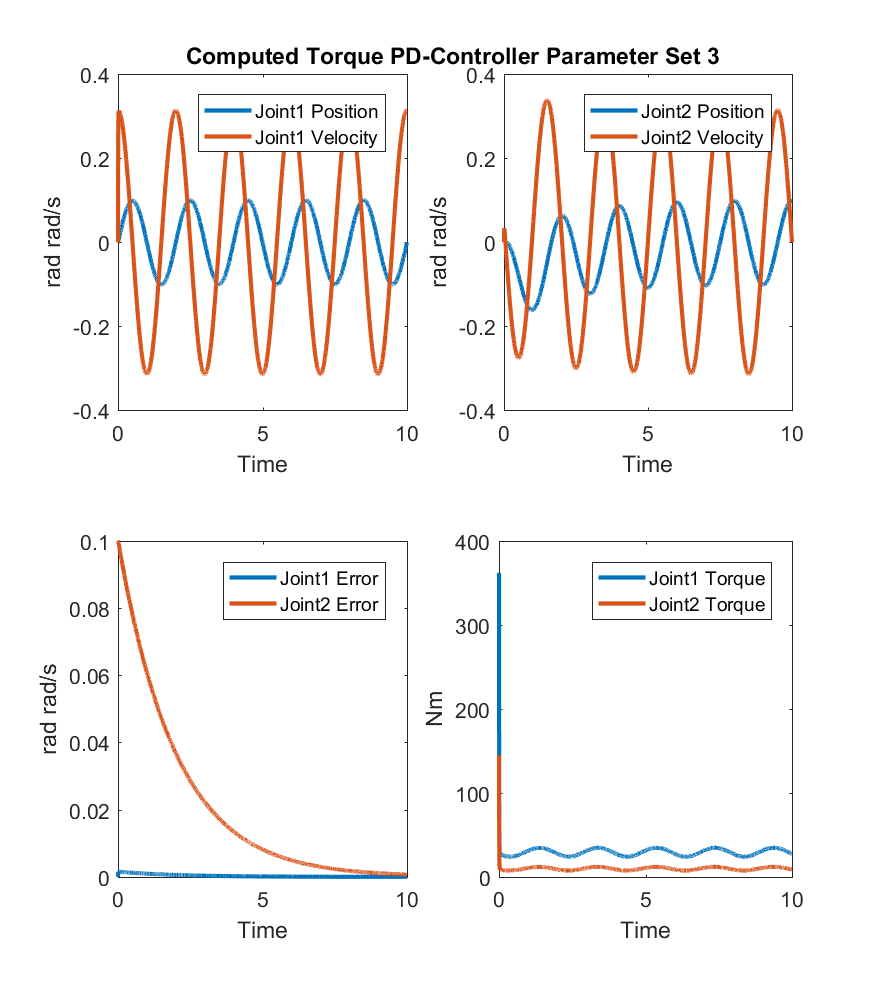
\includegraphics[width=0.85\textwidth]{pics/ComputedTorquePD-ControllerParameterSet3.png}\\
	\caption{Computed Torque PD Controller with over-damping}
	\label{fig:ct_pd3}
\end{figure}

The last simulation uses the parameter set from the first simulation, so the critically damped controller. Although here is a distortion torque applied to each joint. Since the controller is based on a PD-setup, the closed loop answer is not expected to have no steady-state error. In figure \ref{fig:ct_pd4} exactly this behavior can be seen. The other signals are visually the same as the initial simulation with the same parameter set. To avoid the steady-state error another control approach needs to be chosen.
\begin{figure}[]
	\centering
	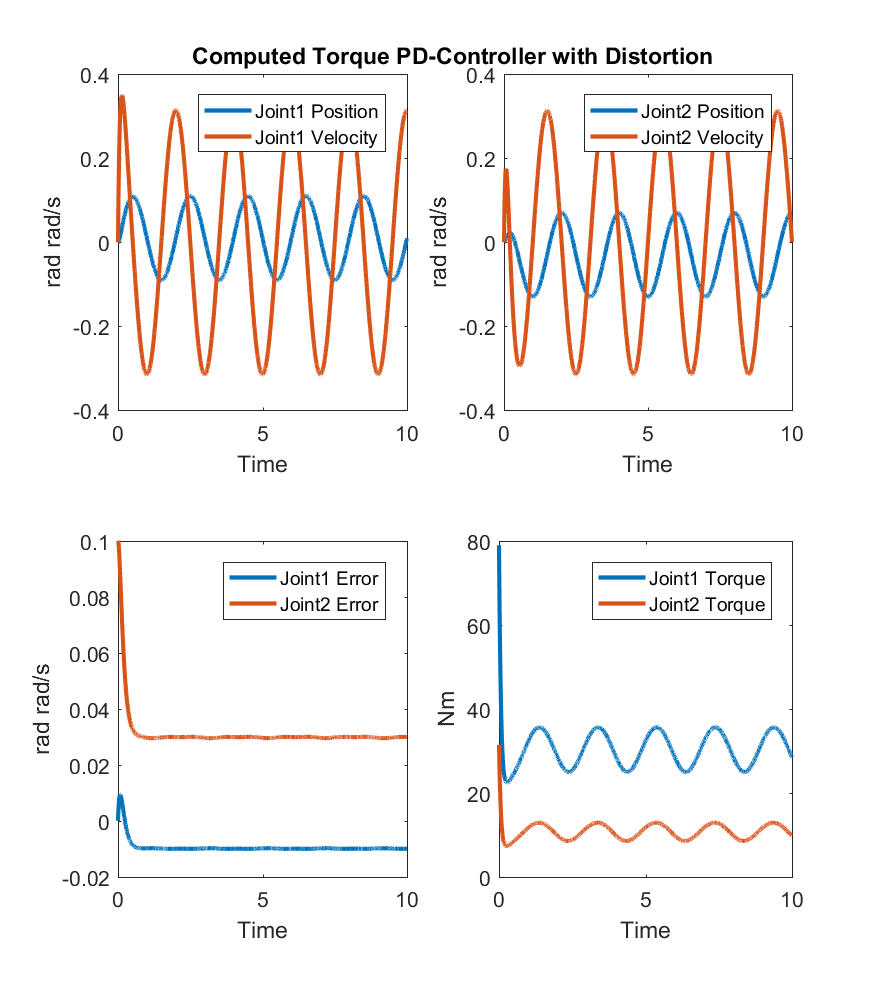
\includegraphics[width=0.85\textwidth]{pics/ComputedTorquePD-ControllerwithDistortion.png}\\
	\caption{Computed Torque PD Controller with distortion}
	\label{fig:ct_pd4}
\end{figure}

\section{PID-Controller}

Similar to the previous approach a controller can be designed using a PID control structure.

\begin{gather*}
\mathbf{u} = -\mathbf{K}_d \dot{\mathbf{e}} - \mathbf{K}_p \mathbf{e} - \mathbf{K}_i \mathbf{\varepsilon}
\intertext{where:}
\varepsilon \int \mathbf{e(\tau)}\mathrm{d}\tau
\end{gather*}

It can shown that the characteristic polynomial of the system is given by: 
\begin{equation*}
\Delta(s) = s^3 + k_{d}s^2 + k_{p}s + k_{i} = 0
\end{equation*}

To calculate the conditions, for which this polynomial only contains negative roots, the Routh-Hurwitz stability criterion is used.
\begin{gather*}
\begin{tabular}{>{$}c<{$}>{$}c<{$}>{$}c<{$}}
1 & k_{p} & 0 \\
k_{d} & k_{i} & 0\\
\dfrac{k_{d}k_{p}-k_{i}}{k_{d}} & 0 & 0\\
k_{i} & 0 & 0
\end{tabular}
\end{gather*}
In order, that the first row has no changes in sign, the following conditions need to be fulfilled:
\begin{align*}
k_{d} &> 0\\
k_{i} &> 0\\
k_{p} &> \frac{k_{i}}{k_{d}}
\end{align*}

The controller gain $k_i$ is given with 500. By parameter coefficient comparison with the characteristic polynomial this leads to $k_p = 2520$ and $k_d = 100.2$.\\

\begin{figure}[]
	\centering
	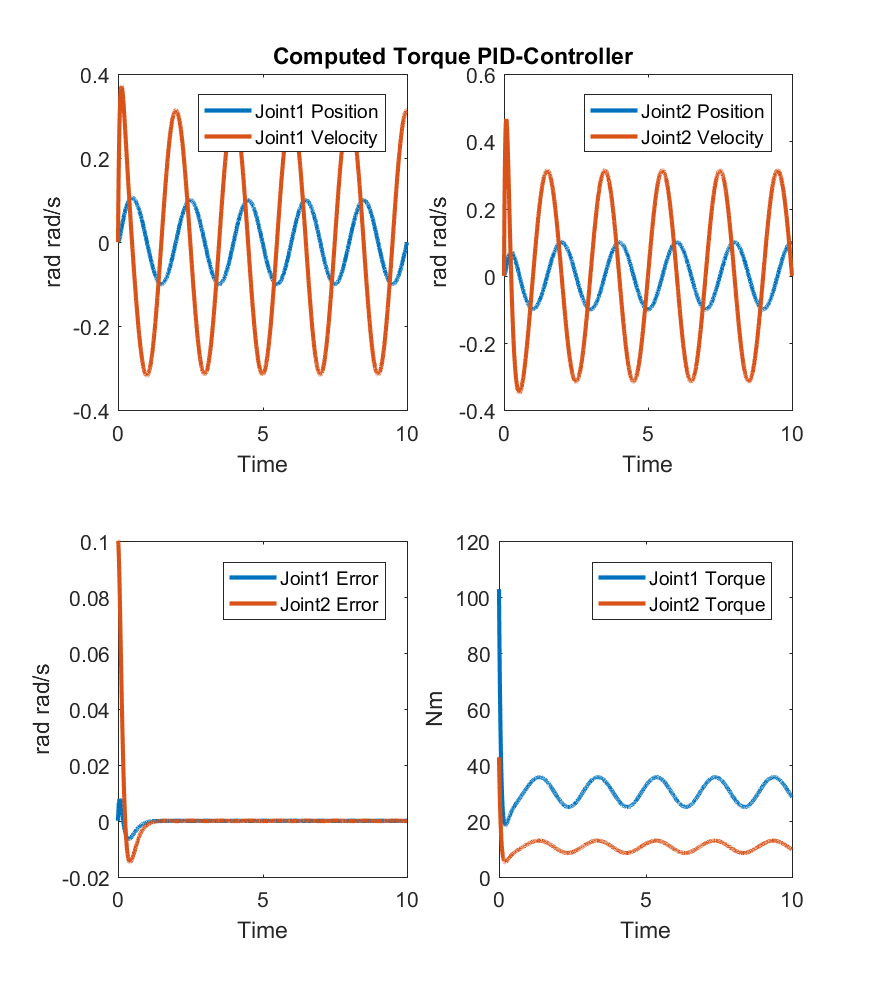
\includegraphics[width=0.85\textwidth]{pics/ComputedTorquePID-Controller.png}\\
	\caption{Computed Torque PID Controller}
	\label{fig:ct_pid1}
\end{figure}


The robot arm is simulated with this type controller and a disturbance of 1Nm at each joint. The results of this simulation can be seen in figure \ref{fig:ct_pid1}. The values of torque and the behavior of the error dynamics is comparable to the critically damped PD-Controller, although this system is able to handle the distortion of the joints, since it was an integrator within the controller. This integrator allows the closed loop answer of the system to have no steady-state error.\\
\begin{figure}[]
	\centering
	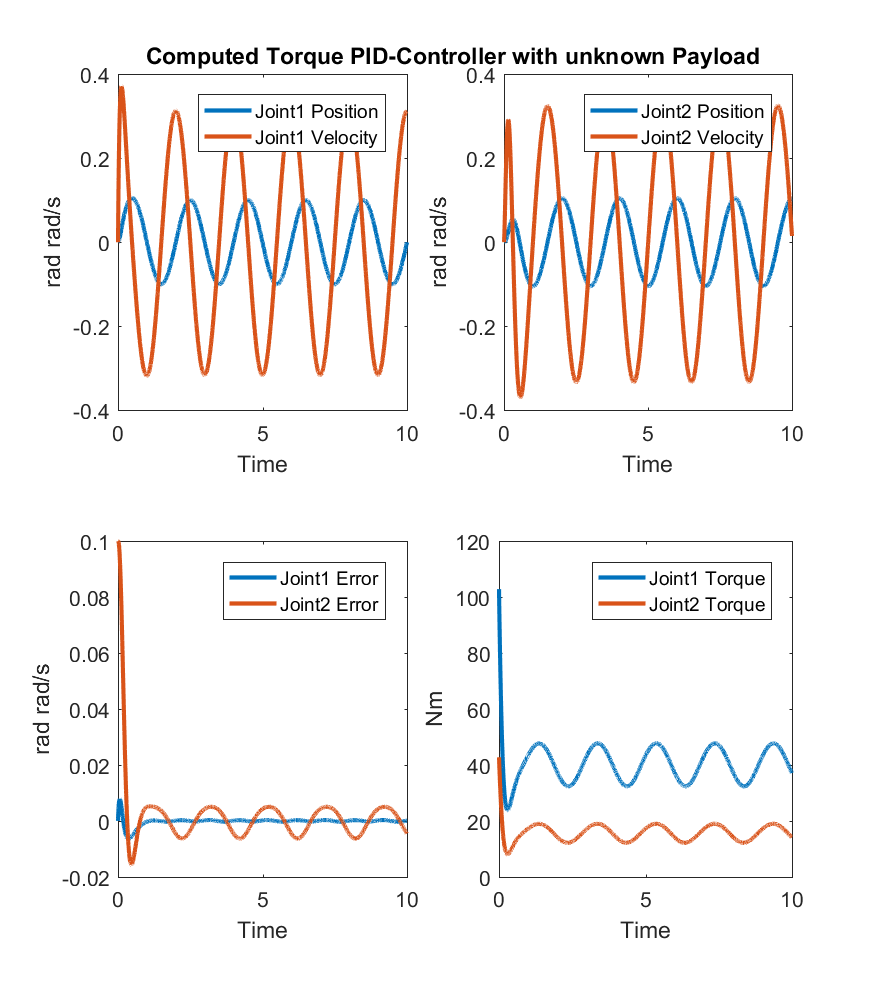
\includegraphics[width=0.85\textwidth]{pics/ComputedTorquePID-ControllerwithunknownPayload.png}\\
	\caption{Computed Torque PID Controller with unknown Payload}
	\label{fig:ct_pid2}
\end{figure}\\
The  simulation of figure \ref{fig:ct_pid2} uses the same controller setup and parameter as the previous simulation, although the robot model itself has been changed, by applying an known payload to it. The controller is not aware of this change and this can be seen within the dynamics of the system. The error of the seconds joint starts to oscillate, where the previous simulation show no steady state error at all.

